%Observação importante: para usar os recursos da classe ABNTEX, é necessário fazer o download de sua biblioteca,
%visto que a mesma não é nativa do ambiente \LaTeX.
%Em um distribuição linux baseada em debian o pacote pode ser instalado pelo comando: sudo apt-get install abntex.
%Autor:Jean Henrique Ferreira Freire

\documentclass{abnt}
\usepackage[brazil]{babel}
\usepackage[utf8]{inputenc}
\usepackage[num]{abntcite}
\usepackage{graphicx}
\usepackage{url}

\begin{document}
\autor{Vitor Botelho Vaz de Melo}

\titulo{Identificando Linhas de Códigos Comentadas em Repositórios de Software}

\orientador[Orientador:\\]{André Hora - Departamento de Ciência da Computação}




\comentario{Proposta de Projeto de Pesquisa e Tecnológico da disciplina de Projeto Orientado em Computação do DCC/UFMG}

\instituicao{Universidade Federal de Minas Gerais \par Instituto de Ciências
Exatas \par Departamento de Ciência da Computação}

\local{Belo Horizonte} \data{2019/1}

% \capa 

\folhaderosto 


% \begin{resumo}
% Coloque aqui seu resumo.\\


% \textbf{Palavras-chaves}: palavras, chave. 
% \end{resumo}

% \sumario %comando que gera o sumário automaticamente
% \renewcommand*\listfigurename{LISTA DE FIGURAS}
% \listoffigures %comando que gera um sumário para a lista de figuras do texto automaticamente



\chapter{INTRODUÇÃO}

À medida que a Ciência da Computação avança e milhões de linhas de códigos são 
escritas, diariamente e em diversas linguagens de programação, os desenvolvedores 
percebem que, para alcançar sucesso a médio e longo prazo em seus projetos, é
necessário utilizar-se, cada vez mais, das melhores ferramentas e práticas de 
programação. 

Uma prática de programação muito comum ao se desenvolver softwares é a de 
''remover'' uma linha ou um bloco de código tornando-os comentários, sendo conhecida  
como commented-out code. Comentar uma linha de código pode ser útil, tanto que 
os próprios ambientes de programação (IDE's e editores de texto) oferecem atalhos 
fáceis para isso. Contudo, esta prática se torna um verdadeiro problema quando 
estes códigos comentados estão inseridos em um sistema grande, complexo e
mantido por diversas pessoas.

A inserção de código comentado nos arquivos fontes de um sistema pode causar
redução da legibilidade, distração e perda de tempo. Martin, em seu livro clássico
Clean Code, enfatiza \textit{"Few practices are as odious as commenting-out code. 
Don’t do this!"}, ele argumenta que outras pessoas não terão coragem de deletar 
este código por achar que ele pode ser importante. 

Além disso, quando um mantenedor se depara com códigos comentados ele pode ter uma 
série de dúvidas, como \textit{"Por que este código está comentado? Isso é útil em 
alguma função? Este código está relacionado com determinada mudança?"}, entre outras 
questões específicas para cada sistema. Este tipo de reflexão pode no mínimo ser 
uma perda de tempo, ou até mesmo uma distração para introduzir bugs no sistema.

No entanto, existem poucos estudos científicos abordando esta problemática e não 
há, entre as ferramentas mais populares, uma solução que identifica automaticamente
este tipo de comentário. Portanto, este trabalho tem como objetivo o desenvolvimento
de uma ferramenta apropriada utilizando técnicas de aprendizado de máquina e, a partir
disso, fazer um estudo abrangente dessa prática em repositórios de código aberto.


\chapter{REFERENCIAL TEÓRICO}


\section{Commented-out code}

\begin{figure}[h!]
  \centering
  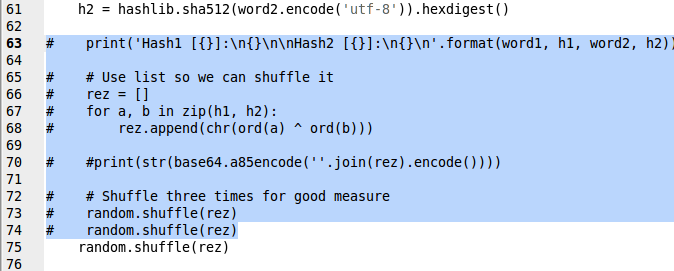
\includegraphics[height=2.4in,width=6.3in]{images/gcc06.png}
  \caption{Commented-out code example}
  \label{fig:commentExample}
\end{figure}

\section{Mineração de Repositórios de Software}

\section{Aprendizado de Máquina}

\section{Algoritmos de Classificação}

\section{Trabalhos Anteriores}

(no trabalho anterior foi obtido um índice de acerto de 85\% com parses
heurísticos para a linguagem java, portanto, essa é uma taxa que esperamos
superar neste trabalho)

\chapter{METODOLOGIA}

\section{Extração e Preparação dos dados}

Deverá ser extraído de diferentes repositórios de software todos os tipos
de comentários. Em sequência estes comentários devem ser classificados 
manualmente como commented-out code (1) ou comentário normal (0) a fim de se formar 
uma base de treinamento. Esta base deverá contemplar diferentes tipos
de linguagem para que o classificador consiga identificar códigos
comentados independente de linguagem. Dessa forma teremos uma base de dados em que o X será igual a uma linha de
comentário e o Y igual a 0 se for um comentário normal ou 1 se for um 
código comentado, que servirão, respectivamente, como input e output para 
o treinamento do classificador.

\section{Treinamento de Modelos de Classificação}

Nesta etapa selecionaremos uma variedade de modelos/algoritmos de classificação,
como por exemplo redes neurais multi-layer perceptron, LSTM, etc. com o 
objetivo de encontrar um classificador com alto índice de precisão 
. Para compararmos os classificadores será 
computado os índices de precisão (True Positive Rate) e revocação
(False Positive Rate) de cada modelo.


\section{Compilação de dados de Repositórios}

Com a ferramenta de identificação de códigos comentado preparada será analisado 
diversos repositórios de softwares de código aberto, encontrados
no GitHub. Ao identificar os comentários será possível calcular a taxa de 
código comentado em relação ao total de comentários em uma versão do 
software e com o auxilio da ferramenta Git será analisado a evolução do 
software através do código de diferentes versões, com isso teremos 
indícios de como os desenvolvedores estão lidando com essa prática, entre 
diversas outras informações que podem ser explorada com este tipo
de técnica.

\chapter{RESULTADOS ESPERADOS}

Espera-se que ao final da disciplina POC I se tenha uma ferramenta robusta e
com alto nível de precisão para identificar códigos comentados em diversas
linguagens de programação. No final da disciplina POC 2
espera-se compreender como a má prática de remover código através de 
comentário afeta a evolução dos diferentes repositórios de código aberto.

\chapter{ETAPAS E CRONOGRAMAS}

\bibliography{references.bib}

\end{document}
